% Extension 2: CP-Decomposition Slides

\begin{frame}{Extension 2: CP-Decomposition}
    \begin{columns}
        \column{0.5\textwidth}
        \textbf{Motivation:}
        \begin{itemize}
            \item Post-hoc $\to$ \textbf{intrinsic} interpretability
            \item Standard eigendecomposition: orthogonality $\to$ entangled
            \item CP: disentangled features
        \end{itemize}
        
        \vspace{0.2cm}
        \textbf{CP Factorization:}
        \begin{equation*}
            W_{cij} = \sum_{r=1}^{R} \lambda_r A_{cr} B_{ir} C_{jr}
        \end{equation*}
        
        \vspace{0.2cm}
        \textbf{Key Properties:}
        \begin{itemize}
            \item No orthogonality constraint
            \item Disentangled representations
            \item Parameter reduction: $\mathcal{O}(R \times d_{\text{in}})$
        \end{itemize}
        
        \column{0.5\textwidth}
        \begin{figure}
            \centering
            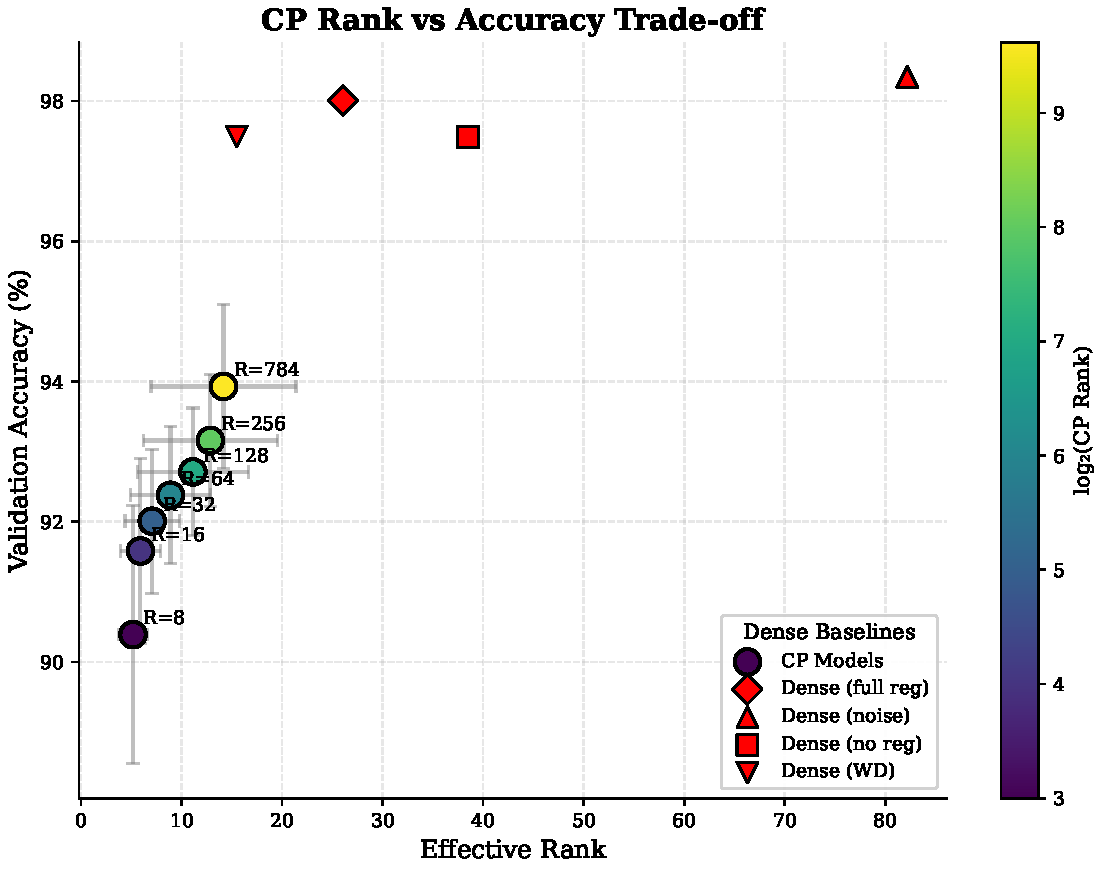
\includegraphics[width=0.95\textwidth]{../Report/figures/extension_cp/cp_rank_accuracy_tradeoff.pdf}
            \caption{Accuracy vs rank trade-off}
        \end{figure}
        
        \vspace{0.2cm}
        \textbf{Results at $R=256$:}
        \begin{itemize}
            \item Accuracy: \textbf{93.8\%}
            \item Effective rank: \textbf{17.5}
            \item vs Dense: 97.5\% (3.7 pp drop)
        \end{itemize}
    \end{columns}
\end{frame}

\begin{frame}{CP-Decomposition: Disentangled Factors}
    \begin{figure}
        \centering
        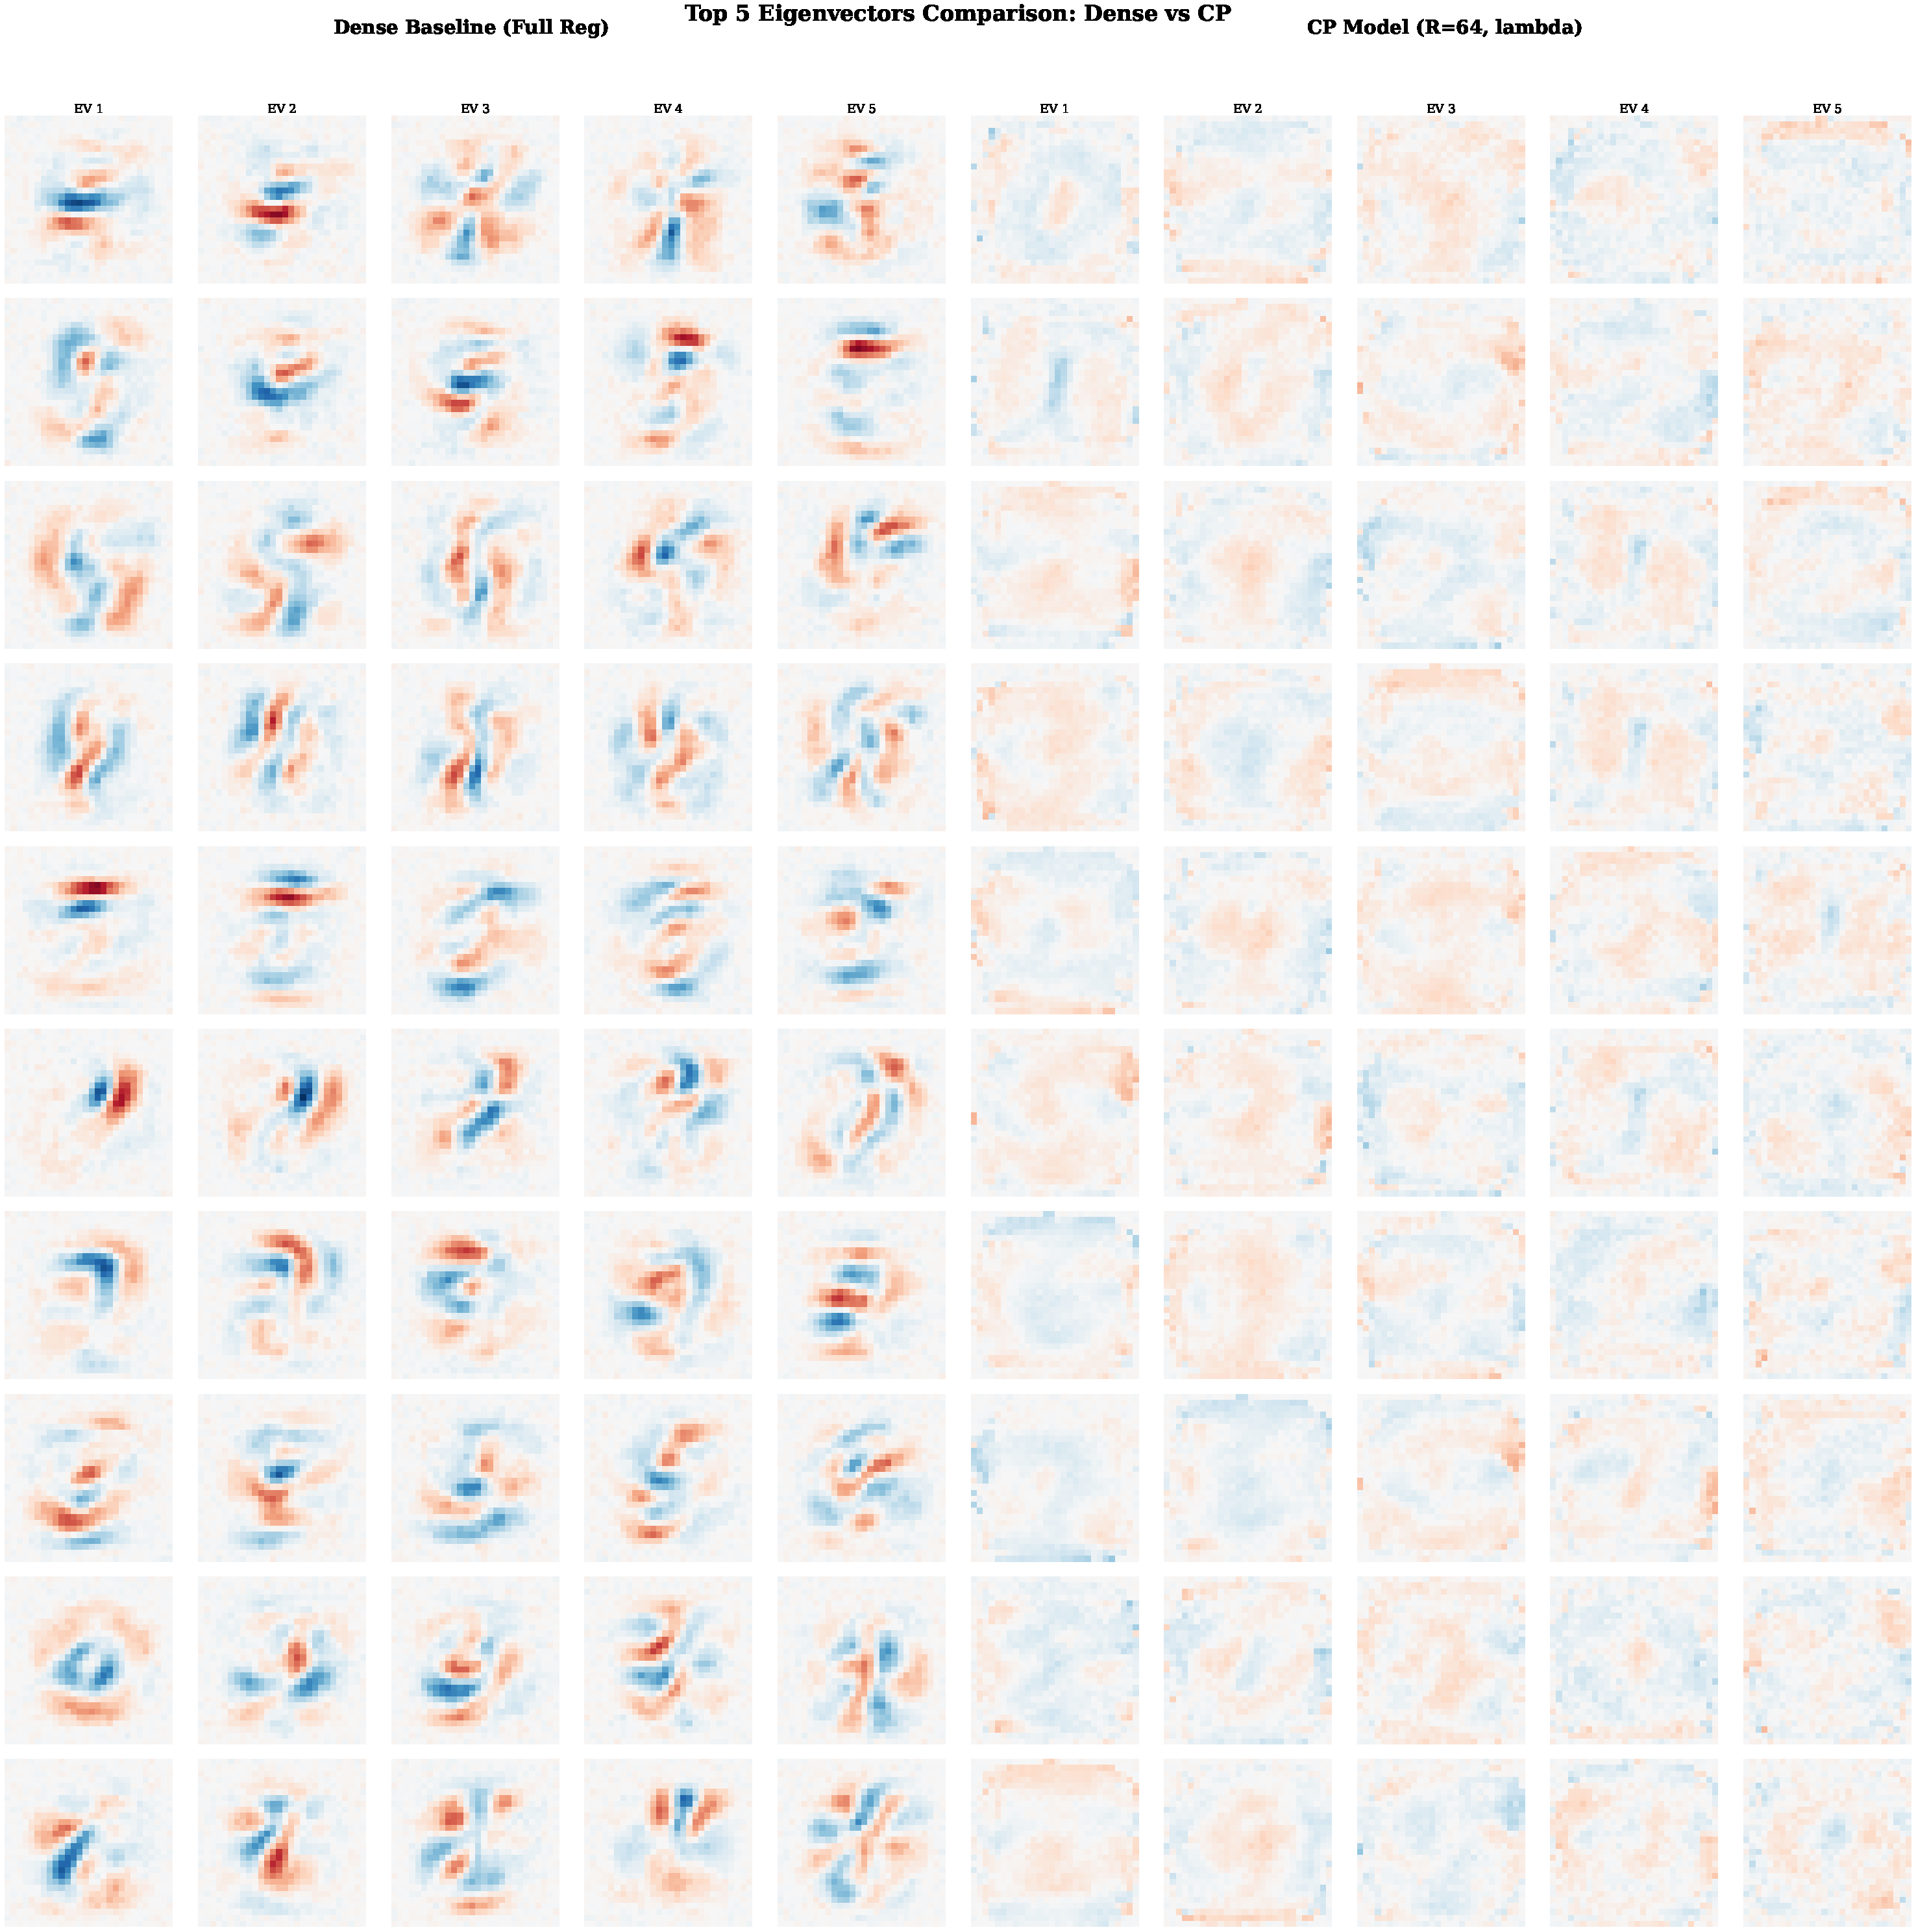
\includegraphics[width=0.8\textwidth]{../Report/figures/extension_cp/cp_top5_eigenvectors_comparison.pdf}
        \caption{Feature disentanglement: Dense vs.\ CP}
    \end{figure}
    
    \vspace{0.2cm}
    \begin{columns}
        \column{0.5\textwidth}
        \textbf{Dense Eigenvectors:}
        \begin{itemize}
            \item Holistic, superimposed templates
            \item Mixed multiple strokes
            \item Entangled representations
        \end{itemize}
        
        \column{0.5\textwidth}
        \textbf{CP Factors:}
        \begin{itemize}
            \item Atomic, localized factors
            \item Isolated curves, specific strokes
            \item Linearly combinable
            \item ``Parts-based'' representations
        \end{itemize}
    \end{columns}
\end{frame}
